The purpose of this thesis was to create a mobile app for managing key features of the KEMS. The KEMS is implemented in the .NET framework, as well as our back-end CAPI app which was created as an extension to KEMS. For faster development of the API we decided to utilise the active server pages (ASP) .NET's library Web API 1.0. The implementation of the CAPI architecture was influenced by \linebreak[4] the representational state transfer (REST) architecture. Our mobile app had to be offering simple graphics, therefore we expected low performance requirements and we wanted to support as many platforms as possible at the same time. We concluded the Apache Cordova framework (ACF) to be the most appropriate tool for the task. As for the functionality of the mobile app the library JS Query (JQuery) was used and for asynchronous communication with the back-end Ajax was utilised. To achieve better results in the presentation aspect another JS library called JQuery Mobile(JQM) was used. The communication between the CAPI and KenticoApp in ensured by the JSON format.

In this chapter we will describe KEMS which is the system extended by this thesis. Next are web APIs and their architectures, \linebreak[4] in particular REST architecture will be introduced. Later we will talk about mobile apps, the ACF and the languages used for the development in this framework, which are CSS, HTML and JS. Lastly Ajax and JSON will be detailed. 
\section{Kentico EMS} \label{analysisKenticoCMS}
KEMS \cite{kentico-product-overview} is a content management system (CMS) which allows clients to create and manage their web-sites using a single user interface (UI) which is made of tiles, a layout and an edit button as can be seen in the image \ref{kentico9UI}. Each tile has its own functionality and the functionality of the tiles in the red circle is implemented in KenticoApp. \linebreak[4] This image was created via print screen from the administration interface of the Kentico 9.0 product.

The client can rearrange them either by simply dragging them or by pressing the edit button. Pressing the button leads to the tiles having an \textit{X} in the upper-right corner for removing the tile. If place on the dashboard is available, a blank rectangle with a plus in the position of the future tile enables the client to add a new tile from the menu. 

\begin{figure}[ht!]
  \centering
  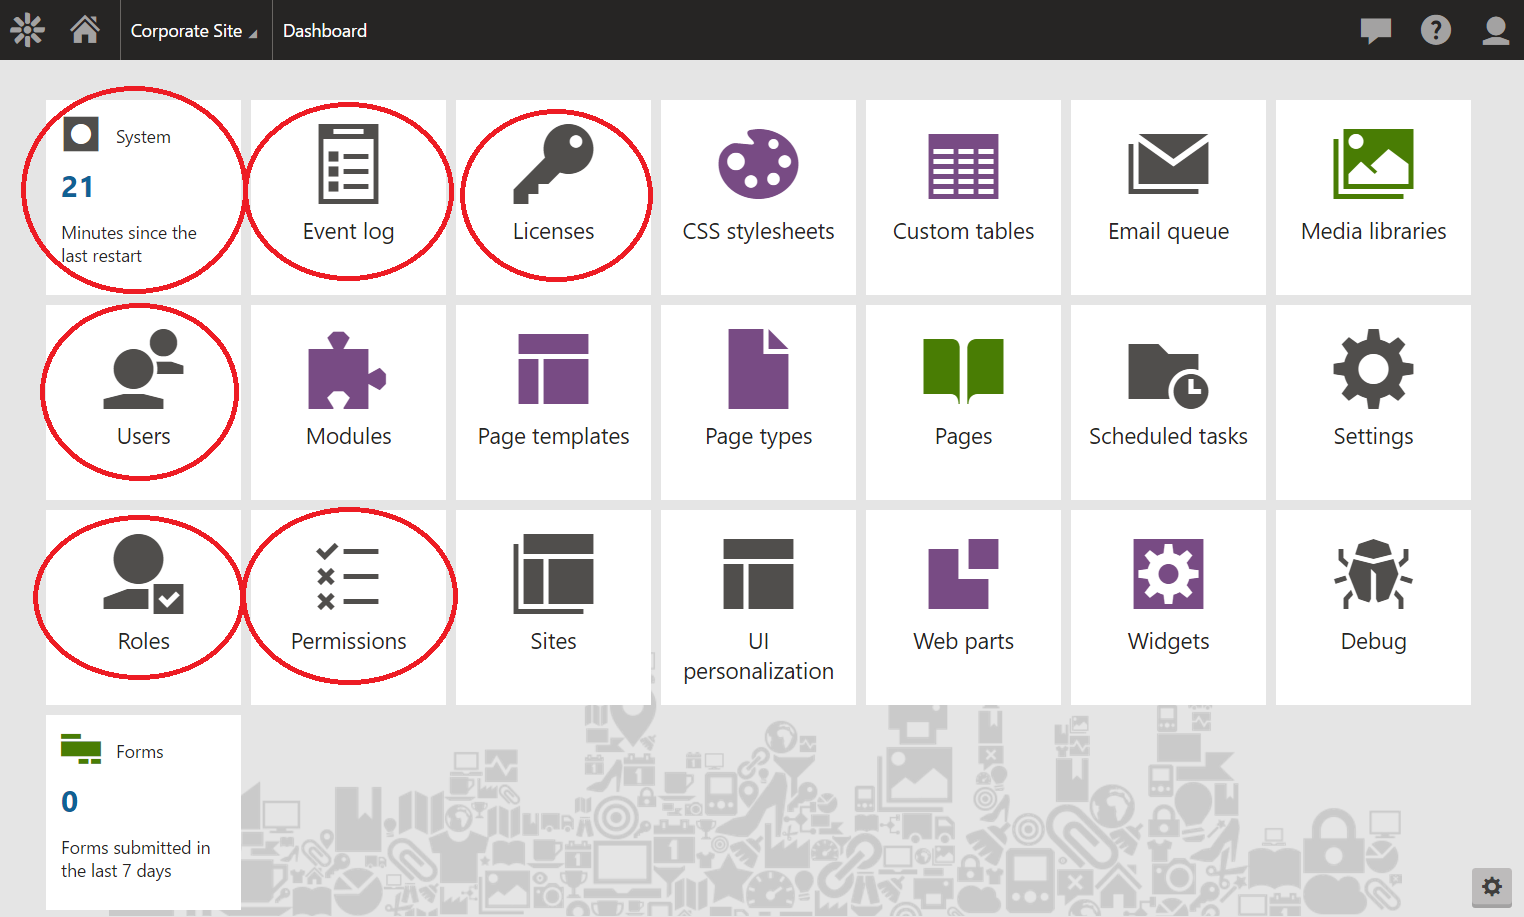
\includegraphics[width=\textwidth]{Images/Kentico9.png}
  \caption{Kentico 9.0 UI. Modified for illustrational purposes.}
  \label{kentico9UI}
\end{figure} 

The functionality in the menu is divided into six categories, namely: Content Management, On-line Marketing, E-Commerce, Social \& Community, Development and Configuration. 
\begin{description}
\item [Content Management] sees to the contents of the client's site such as pages, tables, polls, etc. 
\item [On-line Marketing] enables the client to handle marketing elements. Visitor's behaviour and reactions are taken into consideration. The tiles to be chosen are Email marketing, MVT Tests, Personas and others. 
\item [E-commerce] offers actions which lead to motivating the visitor's behaviour to resemble the client's wished one, managing products and to track sales. These action are for example Buy X get Y discounts, Products and Store reports. 
\item [Social \& Community] makes it possible for the client to maintain the community around the site and its communication. Some of these tiles are for instance Avatars, Chat, Events. 
\item [Development]'s task is to empower the client to administer sources of functionality and programmable elements. This section consists of tiles such as CSS stylesheets, Email templates, Web Part Containers, etc. 
\item [Configuration] The last, in this thesis most important category. This category mostly oversees the overall configuration of the Kentico server. It contains the key requirements of KenticoApp.
	\begin {description}
	\item [System] One of those requirements is the System tile. Part of the System are several subcategories. The one of interest, however, is the one called General. It shows general information about the system and system time, the database and statistics of memory, garbage collection, cache and page view. The default value of the refresh interval is 1 second. It can be changed to up to 60 seconds. Other services General provides are Restart application, Clear cache, Clear performance counters and Clear unused memory. 
	\item [Eventlog] is another key feature. It offers a dropdown list of available sites, a list of events, a filter to view specific events and a button to clear the log. 
	\item[Licenses] the purpose of tile is to show and add licenses of the client and their details. It also allows the client to Export list of domains. 
	\item [Users] grants the ability to view, add and edit the users, monitor the on-line ones and send mass emails. A filter tool is at service for searching users.
	\item [Roles] Users are assigned with roles and this is where these roles are administered. The overview displays all of the site's roles end their details. The client is able to add, edit and delete roles. A dropdown with sites to be chosen is present. 
	\item [Permissions] Roles authorize users to execute certain actions. Permissions define what these actions are. They are managed in this tile. Again, filter options and a dropdown with site names are available. 
	\end{description}
\end{description}
More functionality can be added to the KEMS app by using already created modules or by developing new ones from scratch since it is an extensible system.

\section{Web API} \label{analysisWebAPI}
An~API is a~collection of~functionality which a~programmer is able to~utilise in a~third party app. A web API is an API intended for utilisation by a web server or browser. APIs can be implemented following certain architectures, e.g. REST.
\subsection{REST architecture} \label{analysisREST} \cite{rest}
REST is an architecture of client-server communication based on the dissertation of Roy T. Fielding \cite{fieldingDissertation}. We decided to be inspired by this architecture since most modern APIs are supported by it. It offers constraints and conventions and the programmer has to decide whether they will be followed or not. 

\cite{hateoas} Hypermedia as the engine of application state (HATEOAS) is one of those restrictions. It demands the API is completely hypermedia driven which means a change of state is achieved using hyperlinks. After sending a request, the returned file contains the wanted commodity but also information about how it can be handled. \linebreak[4] An example of a HATEOAS response using JSON format is below. JSON will be described later \ref{analysisJson}.
\lstset{style=sharpc, numbers=none}
\begin{lstlisting}
{
  "id":42, "links":[{ 
	"self":{"href":"/students/42"}, 
	"timetable":{"href":"/timetables/42"}}]
}
\end{lstlisting}
The response contains the student with the ID 42 and links to \linebreak[4] the student itself and to their timetable. 

APIs built using REST leverage most commonly JSON format and are lightweight. This means they operate with simple data representation and therefore the delay between sending and delivering is comparatively small. The client needs no knowledge of how the server is built. It depends on the resources (nouns) and operations (verbs). Hyper text transfer protocols (Http) status codes (SC) can be returned after executing the verbs \cite{rfc-2616}. The nouns are identified with Universal Resource Identifiers (URIs). Each URI represents only one noun. \linebreak[4] The system returns a SC depending on the success of the request. If it is unsuccessful the SC returned gives away the reason why \linebreak[4] the call failed and might carry additional information. Some of \linebreak[4] the most common usage of the most utilised SCs is described below \cite{httpmethods}.
\begin {description}
\item [200 OK] SC means the request was successful and the data have been returned. SC \textit{204 No Content} represents the same meaning but returns nothing.
\item [201 Created] is used when the request was successful and the resource was created. It should return a link to the resource created.
\item [400 Bad Request] is returned when the given parameters were invalid. A reason might be added in the error message. The call should be repeated with different parameters.
\item [401 Unauthorized] it transmits the information the user should try and sign in again. It is meant to be returned if the client is not signed in or does not have the needed permissions. However, it mostly is returned if the user is not authenticated.
\item [403 Forbidden] its purpose is to let the user know not to repeat the request. It is meant to be returned if the client is authorized and authenticated but the system refuses to execute the call but it is most often applied in case the client is not authorized to execute a specific call.
\item [404 Not Found] is shown if a resource is not found with the given URI and it is unknown how long this condition will remain. It can be used if the reason for the failure remain unknown or a resource has to be hidden. Also this is the SC which is applied if no other code is suitable.
%\item [500 Internal Server Error] is returned if the server failed the call due to an unexpected event. 
\item [503 Service Unavailable] SC means the server is not able to fulfill the request at the moment. It is utilised when maintaining the server or overloading it.
\end{description}	
The most applied verbs are described using the following keywords: \textit{OPTIONS}, \textit{GET}, \textit{POST}, \textit{PUT}, \textit{PATCH} and \textit{DELETE}. For the description of them we provided two example URIs:

\begin{enumerate}
\item 
\lstset{style=sharpc}
\begin{lstlisting}
http://example.com/students/47
\end{lstlisting}

\item 
\lstset{style=sharpc}
\begin{lstlisting}
http://example.com/students
\end{lstlisting}
\end{enumerate}

\begin {description}
\item [OPTIONS] offers information about what verbs can be invoked upon a noun. The first URI example with the prefix \textit{OPTIONS} returns all of the bellow verbs. 
\item [GET] is used to read data from the server. It is read only, data must not be changed. The SCs it returns are \textit{200}, \textit{400} and \textit{404}. The first URI example with the prefix \textit{GET}returns the student with the ID 47.
\item [POST] is mostly utilised to create data. It returns SCs such as \textit{201}, \textit{400} or \textit{404}. The second URI with the prefix \textit{POST} creates a new student and returns the resource's location.		
\item [PUT] is most commonly leveraged for updating resources with the sent data. The data are a representation of the complete resource. It returns SCs \textit{200}, \textit{204} and \textit{404}. The first URI edits the student with the id 47.
\item [PATCH] is mostly used for modifying resources. The difference between PATCH and PUT is the sent data can be described by only a part of the resource that needs to be changed. It returns the same SCs as \textit{PUT}. The first URI with the prefix \textit{PATCH} modifies the student with the ID 47.
\item [DELETE] deletes the resource. It returns the status codes \textit{200} and \textit{404}. The first example URI with the prefix \textit{DELETE} deletes the student with the id 47.
\end{description}
Each verb can be shared among multiple nouns. However, each noun might not be able to use each verb. For example an AT usually is not updated, therefore the verb \textit{PUT} is not used with the AT resource.

The platform is not relevant in the implementation when using API's with REST principles. The client and server can even be built on different platforms. This is the reason why it is widely used in web apps. The session between the client and server is stateless, which means the server does not store the client's state. Instead it generates an AT which is sent to the client. This is an advantage since the client is enabled to communicate with different servers or machines in one session. Another benefit is if the server has to be restarted no data of the client's state are lost. It also makes the system highly scalable. REST is an alternative to Simple Object Access Protocol (SOAP), which is more complicated. It has a steeper learning curve. When communicating with SOAP services the client app reads the web service definition language (WSDL) file which contains the description of the functionality supported by the service. REST relies on conventions, therefore this step is omitted. SOAP usually operates with Extensible Markup Language (XML). It has its own advantages in case of large enterprise systems as opposed to REST which is mostly used when building web apps, as already stated.

\section{Mobile applications} \label{analysisMobileApplications}
The client app we are developing in this thesis is running on mobile devices. Mobile apps are more important every day since \textit{no other technology has impacted us like the mobile phone. It's the fastest growing manmade phenomenon ever -- from zero to 7.2 billion in three decades}\cite{more-gadgets-on-earth-than-people}. The platforms, on which these apps run on, can be divided into three main categories: Android, iPhone OS (iOS) and the Windows family of operating systems for mobile devices (WM). The most used operating system (OS) with a share of 68.67\% of all mobile devices as of November 2016, according to \textit{netmarketshare.com} \cite{operating-system-market-share} is Android. It was  released in September 2008 and its native language is Java. With a percentage of 25.71\%, iOS is the second most sold mobile OS and was released in June 2007. Its native language is Swift. The third platform is WM with 1.75\% share. It was first released in November 2010 and the native language is C\#. 

Mobile apps can be divided into three types: Native, HTML5 and Hybrid.
\begin {description}
\item [Native] This type of app is written in the native language of the platform the developer wants to target. It is fast and the behaviour is most intuitive for its users because the developer focuses on one particular OS and its features. The drawback is that for the development of a native app the learning curve is steep which is why an experienced team of programmers is needed and it targets only one OS. If the app has to run on other platforms, it has to be built in their native languages. This is time costly and therefore expensive. 
\item [HTML5] These apps run in a devices browser. They are usually implemented in CSS, HTML and JS. Many programmers have the opportunity to leverage their previously acquired experience with these languages, alternatively the skills gained here in web programming. HTML5 based apps run slower than native ones but work on multiple OS. This saves time and money. The disadvantage of cross-platform apps is they are less intuitive. For example an app with android features would be uncommon for iOS users and vice versa. Another flaw of this approach is the inability to use the device's hardware, such as its camera or microphone.
\item [Hybrid] This is a combination of the two above. It is primarily built utilising CSS, HTML5 and JS and is \textit{hosted inside a native application that utilizes a mobile platform’s WebView.} \cite{hybrid-mobile-app} The bridge to native technologies is ensured by tools, for example in this thesis the ACF is used. A WebView is a headless browser, without any buttons and without higher level functionality such as tabs, navigation, etc. The perks of this approach is the small learning curve. Thanks to HTML5 it is cross-platform and the native wrapper allows it to use the device's hardware and native API. It still runs slower than Native but is cheaper when more OSs are targeted.
\end{description}

When creating an app the developer has to consider what approach will be the most effective one. If smooth graphical performance is crucial, the app should be native. If it has to run on multiple platforms, make use of a device's hardware component and native API and the graphics are not that important, probably hybrid would be the best fit. If the app displays what was sent to it and has no dynamic graphics then HTML5 should suffice.

The development of KenticoApp was divided into two stages. For the~implementation of the~mobile app we leveraged the ACF, as already stated. The~reason being it is less demanding to learn and supports seven platforms. For creating the UI  we decided to use JQM. It is an~HTML5-based UI framework which allows users to design aesthetically pleasing mobile elements by utilising the~languages CSS and HTML. Document object model (DOM) elements are individual parts of a web page described by tags such as div, span, input or others. These tags assign styling and properties to elements. For the DOM manipulation we used the~JQuery library which has a~small learning curve and offers a~fast way to add, modify, style and delete elements or change their~behaviour. It also offers a set o handy helper functions which provide easy to use interface for frequently used operations in web development, e.g. \textit{ajax()}.

\subsection{Apache Cordova}
ACF is a framework used for creating hybrid mobile apps that are compatible with seven platforms. As opposed to the~Xamarin framework (XF) supporting only three. It allows the programmer to utilise the languages CSS, HTTP and JS. A native wrapper offers the simulation of a native app, meaning the app is able to operate native API through libraries. For example it is able to access the gyroscope information or open the native calendar. XF is used to build native apps in the language C\# on WM, Android and iOS. When launched on Android or iOS its code is translated into Android Java or iOS Swift. Even though XF should be faster than ACF, and therefore offer a smoother user experience, the~difference between execution times of non performance sensitive apps on today's devices is negligible. We did not consider development in native languages because of their steep learning curve and the ability to deploy only to one platform.
\subsection{HTML, CSS, JS}
These languages are the most common ones in front-end web programming. HTML is a markup language and is used to define the structure of a page. CSS is leveraged to add styles, such as colors, fonts or alignment. JS adds functionality to a page. Because there are nuances between different browsers and browser versions it can be time consuming to create a page using only these languages. Therefore a framework is typically used to simplify these tasks, providing its own set of styles, tags and functionalities which are tuned to work in different environments.

\section{Ajax and JSON}
Ajax offers the execution of asynchronous operations. It is able to update a web page without reloading the page. After a page has loaded it can request or receive data from a server and it also is able to send data to a server in the background \cite{ajax-introduction}. This saves time when using an app because the user does not have to wait for a whole page to load again. Instead, only data of the call have to be awaited. The user can leverage the page before data which take longer loading time, e.g. images are loaded. It is used in browser to server communication.

JSON format \label{analysisJson} is a simple \textit{string}. Attributes are represented with their name, a colon following and the attribute's value. For example \textit{"id":"47"}. If an object is described, the attributes are put into braces. A comma separating them: \textit{\{"id":"47", "type":"student"\}}. If multiple objects are displayed in a \textit{array} the objects are bordered with brackets and again separated by a comma. \textit{[\{"id":"47", "type":"student"\}, \{"id":"007", "type":"teacher"\}]}. This format is not dependent on any platform. JS can manipulate with a JSON file without any conversion which is why it is widely used by front-end web developers.

